\documentclass{article}
\usepackage[letterpaper, total={7.5in, 10in}]{geometry}
\usepackage{graphicx} % Required for inserting images
\usepackage{hyperref}
\usepackage[simplified]{pgf-umlcd}
\usepackage{pdflscape}
\usepackage{xcolor}

\renewcommand {\umltextcolor}{black}
\renewcommand {\umlfillcolor}{white}
\renewcommand {\umldrawcolor}{black}

% \usepackage{emoji}  % LuaLaTeX
% \setemojifont{TwemojiMozilla}

\title{Processing Relay Chat -- PRC}
\author{David Chen -- Team PLA (Pretty Lazy Acronym)}
\date{Period 6}

\begin{document}

\maketitle

\section{Description}
Processing Relay Chat (PRC) encompasses a client program, server program, and protocol for instant messaging over the network. To accomplish this in Processing PRC the \href{https://processing.org/reference/libraries/net/index.html}{Network} library.\\
PRC will include the following features:
\begin{itemize}
    \item Ephemeral plaintext (printable ASCII)\footnote{Due to font limitations, Unicode glyphs for other languages/emojis cannot be fully supported.} messaging
    \item Usernames with deterministic colors
    \item A slash command framework for advanced user interaction
    \item File sharing
    \item Chat log export
\end{itemize}

\subsection{Protocol}
\subsubsection{Packet Format}
PRC uses a JSON-inspired TCP packet schema, in which ASCII separator characters are used, simplifying the burden of packet parsing. Bytes are denoted here using 3-digit octal notation.

Non-printable ASCII, save for the specified special characters, are not permitted in a PRC packet. Row names and data fields may include arbitrary printable ASCII strings (characters ranging from \verb|\040| SPACE to \verb|\176| \verb|~|).

Each row takes the form of \verb|NAME\037DATA|, with \verb|\037| being the "unit separator" byte, analogous to \verb|:| in JSON.
A row can be terminated with the "record separator" character \verb|\036|, analogous to \verb|,| in JSON, to indicate that there is another record to parse, or with \verb|\003|, the "end of text" byte, to terminate parsing. Each row should be processed by the program as a String to String hashmap, with the NAME being the key, and the DATA being the value.

A packet will NOT be parsed until a terminating "end of text" byte is detected.

\subsubsection{Commands}
By convention, commands are represented with a four or five letter, capitalized short string, though arbitrary capitalization, spacing, or length is possible. The command is specified in a PRC packet row named \verb|Command|.

\paragraph{NAME} is the username registration command. The client should provide a \verb|UUID| field, which will be echoed in the response packet, in order to discern whether it is recieving its own name. The client provides the field \verb|User| to describe the requested username, and \verb|Old User| if the client already had a registered username. The server will validate that the username does NOT include \verb|#|, and assign a username of \verb|GuestN|, with $N$ being the number of already registered users, if there is an invalid \verb|User| field. The server will then echo the packet, but with the final, published \verb|User| value.

\paragraph{SEND} is the message send command. The fields \verb|User|, \verb|Content|, and \verb|Channel| are required from the user, and the server will specify \verb|HOST| based on the client's IP address.

\paragraph{JOIN} is the channel join command. The \verb|Channel| field is required, and the server will validate that the channel name does NOT include \verb|#|, and is of appropriate length (18). If the channel has not been created yet, the server will add a new channel to its listing. The server will respond with a \verb|SYNC| packet.

\paragraph{SYNC} is the state synchronization packet. This packet, when sent by the client (or, \verb|CHAN| for backwards compatibility), will request the server to broadcast a \verb|SYNC| packet. The packet contains two fields, \verb|Channels| and \verb|Users|, with \verb|#| to deliminate entries.

\paragraph{QUIT} is the quit command. When a client sends this command to the server, it is requesting a graceful exit, which the server will perform, then send a terminating \verb|QUIT| packet. When a client receives this packet, it will gracefully exit. The server will also send this packet before a server shutdown.

\paragraph{ERROR} is the error packet. The client should never send this packet. The server will send this packet to the client when the client has sent a complete packet containing user errors, and the client should display the packet's contents to the user.

\section{Functionality}
As of right now, message sharing, user color generation, and slash commands are complete. Chat log export and file sharing are to be completed.

\subsection{Issues}
\begin{enumerate}
    \item To share font data among \verb|Text| subclasses, it was appropriate to use \verb|static| variables, but there may be "non-\verb|static| inner type" issues when trying to declare \verb|static| variables in the \verb|Text| abstract class. To fix this, the abstract class itself must be declared \verb|static|. (\href{https://forum.processing.org/two/discussion/23623/when-creating-a-class-what-is-it-an-inner-class-of-declared-static-in-a-non-static-inner-type.html}{Source})
    \item In testing, it appears that a Client and a Server running in the same PApplet may lead to unexpected behavior. Thus, it will be necessary to run the server separately from the client.
    \item The Display class had a tendency for displayed lines to overflow the boundaries of the screen. The solution is to use the bounding box features in Processing's \verb|text()| function to cut off lines as needed, and additional logic to prevent attempted display of additional lines outside of the boundary. To avoid issues with losing message data, it will be possible for the message box to scroll.
    \item The programs would behave erratically if there was a failure to connect to the server or bind to a valid port. To fix this, we can add additional error checks that will attempt to automatically resolve the issue, or prompt the user for corrections.
\end{enumerate}

\section{Log}
\begin{itemize}
    \item 05/20: Began writing program specifications in \LaTeX.
    \item 05/21 -- 05/22: Constructed UML class diagrams for anticipated object classes.
    \item 05/23 -- 05/24: Corrected text location alignment issues.
    \item 05/25: Implemented Text subclasses and display() functions; turned Text into an abstract base class to deduplicate logic; Implemented Display and constructed a testing mockup.
    \item 05/26 -- 05/28: Adjusted UML class designs to provide additional necessary functionality. Began working on network transmission of messages.
    \item 05/29 -- 06/02: Worked around rendering bug that prevented messages from instantly appearing on the screen. Began pondering design and protocol alterations for separate Client/Server classes, along with proper maintainance of message, channel, and user states.
    \item 06/03 -- 06/08: Implemented the network protocol and state-sharing functionality between Client and Server, fixing bugs and pitfalls along the way. Merged the \verb|overflow| branch (from the previously logged step) and implemented scroll buffer features to enable a cohesive user experience. Reassessed scope to fit time frame. Implemented Catpuccin colors anyways because they're neat :)
    \item 06/09: Cleaned up code for improved organization and cohesion in design, updated and rearranged UML diagram from the umpteenth (and hopefully final) time to reflect current classes, documented protocol in detail, began writing plot for planned demonstration skit.
    \item 06/10 (planned):  implementation of final features; script-writing for the demonstration, which I hope to integrate a skit into the demonstration portion, with a broad overview of the code structure, pitfalls along the way, and my personal favorite functions.
\end{itemize}

\begin{landscape}
\section{UML Diagram}
\begin{center}
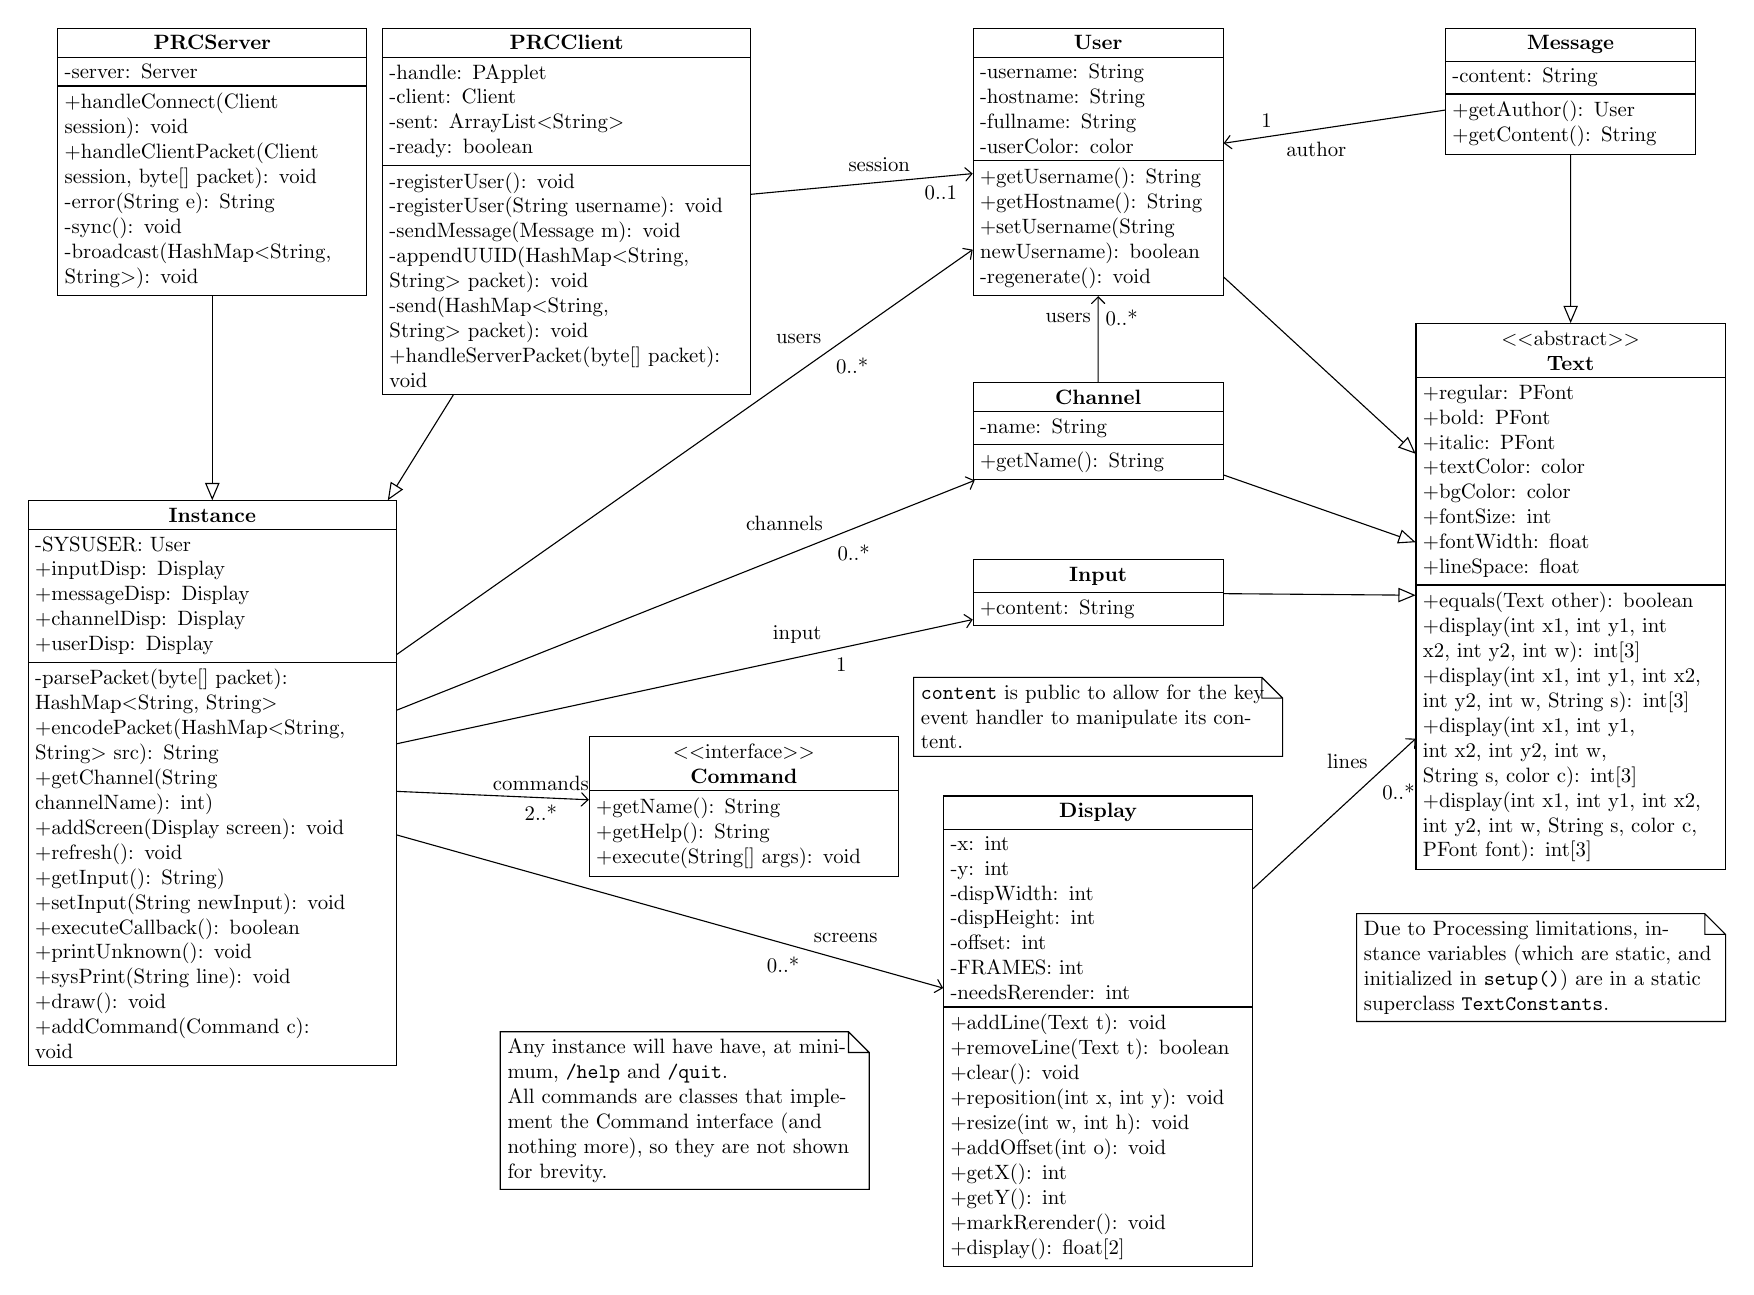
\begin{tikzpicture}
\begin{scope}[scale=0.75, transform shape]
    \begin{abstractclass}[text width = 5cm]{Text}{20,3}
        \attribute{+regular: PFont}
        \attribute{+bold: PFont}
        \attribute{+italic: PFont}
        \attribute{+textColor: color}
        \attribute{+bgColor: color}
        \attribute{+fontSize: int}
        \attribute{+fontWidth: float}
        \attribute{+lineSpace: float}

        \operation{+equals(Text other): boolean}
        \operation{+display(int x1, int y1, int x2, int y2, int w): int[3]}
        \operation{+display(int x1, int y1, int x2, int y2, int w, String s): int[3]}
        \operation{+display(int x1, int y1, int x2, int y2, int w, String s, color c): int[3]}
        \operation{+display(int x1, int y1, int x2, int y2, int w, String s, color c, PFont font): int[3]}
    \end{abstractclass}
	\umlnote[draw, text width = 6cm] at (19.5, -7) (text) {Due to Processing limitations, instance variables (which are static, and initialized in \verb|setup()|) are in a static superclass \verb|TextConstants|.};

    \begin{class}[text width = 5cm]{Display}{12,-5}
        \attribute{-x: int}
        \attribute{-y: int}
        \attribute{-dispWidth: int}
        \attribute{-dispHeight: int}
        \attribute{-offset: int}
        \attribute{-FRAMES: int}
        \attribute{-needsRerender: int}

        \operation{+addLine(Text t): void}
        \operation{+removeLine(Text t): boolean}
        \operation{+clear(): void}
        \operation{+reposition(int x, int y): void}
        \operation{+resize(int w, int h): void}
        \operation{+addOffset(int o): void}
        \operation{+getX(): int}
        \operation{+getY(): int}
        \operation{+markRerender(): void}
        \operation{+display(): float[2]}
    \end{class}
    \unidirectionalAssociation{Display}{lines}{0..*}{Text}

      \begin{class}[text width = 4cm]{Input}{12, -1}
        \inherit{Text}
        \attribute{+content: String}
    \end{class}
    \umlnote[draw, text width = 6cm] at (12, -3) (input-note) {\verb|content| is public to allow for the key event handler to manipulate its content.};

    \begin{class}[text width = 4cm]{User}{12, 8}
        \inherit{Text}
        \attribute{-username: String}
        \attribute{-hostname: String}
        \attribute{-fullname: String}
        \attribute{-userColor: color}
        \operation{+getUsername(): String}
        \operation{+getHostname(): String}
        \operation{+setUsername(String newUsername): boolean}
        \operation{-regenerate(): void}
    \end{class}

    \begin{class}[text width = 4cm]{Channel}{12,2}
        \inherit{Text}
        \attribute{-name: String}
        \operation{+getName(): String}
    \end{class}
    \unidirectionalAssociation{Channel}{users}{0..*}{User}

    \begin{class}[text width = 4cm]{Message}{20, 8}
        \inherit{Text}
        \attribute{-content: String}
        \operation{+getAuthor(): User}
        \operation{+getContent(): String}
    \end{class}
    \unidirectionalAssociation{Message}{author}{1}{User}

    \begin{interface}{Command}{6,-4}
        \operation{+getName(): String}
        \operation{+getHelp(): String}
        \operation{+execute(String[] args): void}
    \end{interface}

    \begin{class}[text width = 6cm]{Instance}{-3,0}
        \attribute{-SYSUSER: User}
        \attribute{+inputDisp: Display}
        \attribute{+messageDisp: Display}
        \attribute{+channelDisp: Display}
        \attribute{+userDisp: Display}

        \operation{-parsePacket(byte[] packet): HashMap$<$String, String$>$}
        \operation{+encodePacket(HashMap$<$String, String$>$ src): String}
        \operation{+getChannel(String channelName): int)}
        \operation{+addScreen(Display screen): void}
        \operation{+refresh(): void}
        \operation{+getInput(): String)}
        \operation{+setInput(String newInput): void}
        \operation{+executeCallback(): boolean}
        \operation{+printUnknown(): void}
        \operation{+sysPrint(String line): void}
        \operation{+draw(): void}
        \operation{+addCommand(Command c): void}
    \end{class}
    \unidirectionalAssociation{Instance}{input}{1}{Input}
    \unidirectionalAssociation{Instance}{screens}{0..*}{Display}
    \unidirectionalAssociation{Instance}{users}{0..*}{User}
    \unidirectionalAssociation{Instance}{channels}{0..*}{Channel}
    \unidirectionalAssociation{Instance}{commands}{2..*}{Command}

    \begin{class}{PRCServer}{-3, 8}
        \inherit{Instance}
        \attribute{-server: Server}

        \operation{+handleConnect(Client session): void}  % serverEvent()
        \operation{+handleClientPacket(Client session, byte[] packet): void}  % Server.available() - server receives packet
        \operation{-error(String e): String}
        \operation{-sync(): void}
        \operation{-broadcast(HashMap$<$String, String$>$): void}
    \end{class}

    \begin{class}[text width = 6cm]{PRCClient}{3, 8}
        \inherit{Instance}
        \attribute{-handle: PApplet}
        \attribute{-client: Client}
        \attribute{-sent: ArrayList$<$String$>$}
        \attribute{-ready: boolean}

        \operation{-registerUser(): void}
        \operation{-registerUser(String username): void}
        \operation{-sendMessage(Message m): void}
        \operation{-appendUUID(HashMap$<$String, String$>$ packet): void}
        \operation{-send(HashMap$<$String, String$>$ packet): void}
        \operation{+handleServerPacket(byte[] packet): void}  % clientEvent() - client receives packet
    \end{class}
    \unidirectionalAssociation{PRCClient}{session}{0..1}{User}

    \umlnote[draw, text width=6cm] at (5, -9) (commands-note) {Any instance will have have, at minimum, \verb|/help| and \verb|/quit|.\\All commands are classes that implement the Command interface (and nothing more), so they are not shown for brevity.};
\end{scope}
\end{tikzpicture}
\end{center}
\end{landscape}
\newpage

\section{Manual}
PRC encompasses two separate programs, a Server and Client program. In both programs, \verb|/help| will print out a description of available slash-commands when they are available.

\subsection{Server Mode}
The server will attempt to start a TCP server on port 2510. If this fails, it will increment upward until a working port is found. If the program fails to find a port, it will exit().

The program will then display an entry screen from which the administrator can use the \verb|/quit| command to disconnect all clients. It will also list the usernames given by user logins, along with the channels that have been created. If the DEBUG boolean is enabled, additional logs will be displayed on screen.

\subsection{Client Mode}
The user will be prompted enter a server address/port to connect to, in the \verb|host:port| format. On successful connection, the user will be registered to a guest username, and join the \verb|#general| chat by default.

Using the \verb|/nick| command, the user can register a username, and using the \verb|/join| command, they are able to change to a different channel, or create their own. Like the server, their screen will display a list of connected users and channels. They can use \verb|/quit| to gracefully exit from the program.

User colors are generated from a palette using a deterministic algorithm that guarantees that the same user with the same nickname on the same host IP address will have the same color as displayed in chat.

Once logged into a channel, the user is allowed to enter their message into the bottom chatbox, and press enter to send it to the channel. This message will only appear when the user has \verb|/switch|ed to the correct channel. Messages in other channels are hidden until the user switches to them.

Using the up and down arrow keys, the user may scroll through chat history, akin to pagers like the \verb|less| command in many Unix environments.

\end{document}
